\documentclass[11pt]{article}
\usepackage[margin=0.8in]{geometry}
\usepackage[T1]{fontenc}
\usepackage{lmodern,microtype,booktabs,graphicx,amsmath,xcolor,hyperref,xurl}
\hypersetup{colorlinks=true,urlcolor=blue,linkcolor=blue,pdftitle={Read reported heat-rate change before making efficiency claims},pdfauthor={James N. Jean IV}}
\setlength{\parindent}{0pt}\setlength{\parskip}{6pt}\setlength{\tabcolsep}{5pt}
\newcommand{\RetainedRows}{27,842}
\newcommand{\NativeSelectedRows}{28,578}
\newcommand{\QuarantinedPlants}{18}
\newcommand{\QuarantinedRows}{736}
\newcommand{\SourceConditions}{814,042}
\newcommand{\ConversionConditions}{55,684}
\newcommand{\ConversionDifference}{7.00E-10}
\newcommand{\GroupRows}{29,996}
\newcommand{\NegativeComponents}{329}
\newcommand{\GroupConditions}{540,314}
\newcommand{\DevCases}{36}
\newcommand{\DevContributions}{36,476}
\newcommand{\DevDeletions}{9,158}
\newcommand{\DevChecks}{658,242}
\newcommand{\HeldCases}{36}
\newcommand{\HeldContributions}{37,636}
\newcommand{\HeldDeletions}{9,814}
\newcommand{\HeldChecks}{682,050}
\newcommand{\MaxDifference}{3.64E-56}
\newcommand{\CoalPlants}{182}
\newcommand{\CoalWithin}{0.039651}
\newcommand{\CoalMix}{-0.005867}
\newcommand{\CoalOutside}{-0.004379}
\newcommand{\CoalChange}{0.029405}
\newcommand{\GasPlants}{1,503}
\newcommand{\GasWithin}{-0.058656}
\newcommand{\GasMix}{0.089560}
\newcommand{\GasOutside}{0.003270}
\newcommand{\GasChange}{0.034174}
\newcommand{\PooledPlants}{1,598}
\newcommand{\PooledWithin}{-0.031403}
\newcommand{\PooledMix}{0.028037}
\newcommand{\PooledOutside}{-0.007434}
\newcommand{\PooledChange}{-0.010799}
\newcommand{\PooledStart}{8.608466}
\newcommand{\PooledEnd}{8.597667}
\newcommand{\PooledCoverageStart}{99.651}
\newcommand{\PooledCoverageEnd}{99.626}
\newcommand{\GasOffsetWithin}{-0.769329}
\newcommand{\GasOffsetMix}{0.828544}
\newcommand{\GasOffsetChange}{0.046282}
\newcommand{\ReplayExact}{615,290}
\newcommand{\ReplayNumeric}{818,646}
\begin{document}
\begin{center}{\LARGE\bfseries Read reported heat-rate change\par before making efficiency claims}\par
\vspace{5pt}{\large Within-cell ratios, generation shares and cohort composition}\par
James N. Jean IV \quad | \quad Independent research program, Study 25 v2\par
October 30, 2026 \quad | \quad Not peer reviewed
\end{center}
\section*{The decision}
A fleet's reported fuel per unit of electricity can change when its cell ratios change, generation moves between cells, or eligible reporting records enter and leave the matched cohort. Before describing a lower fleet ratio as improved plant performance, separate those effects and inspect how individual plants influence the arithmetic.

\textbf{Finding.} In the selected unambiguous pooled coal/gas cohort, the 2023--2024 reported ratio moves from \PooledStart{} to \PooledEnd{} MMBtu/MWh. Its small change of \PooledChange{} contains a within-cell component of \PooledWithin{}, a mix component of \PooledMix{} and an outside-cohort composition remainder of \PooledOutside{}. Opposing terms matter; the headline ratio alone hides them.

\begin{center}\small\begin{tabular}{lrrrrr}\toprule
2023--2024 & Plants$^*$ & Within & Mix & Outside cohort & Net change\\\midrule
Coal & \CoalPlants{} & \CoalWithin{} & \CoalMix{} & \CoalOutside{} & \CoalChange{} \\
Natural gas & \GasPlants{} & \GasWithin{} & \GasMix{} & \GasOutside{} & \GasChange{} \\
Pooled & \PooledPlants{} & \PooledWithin{} & \PooledMix{} & \PooledOutside{} & \PooledChange{} \\
\bottomrule\end{tabular}\end{center}
\smallskip $^*$Matched plant identities. Units: MMBtu/MWh. Rounded components need not add exactly; the full-precision identities are independently checked.

\textbf{Practical recommendation.} Report the ratio, matched-cohort definition, within/mix/remainder terms and finite plant-deletion sensitivity together. If the intended decision concerns physical efficiency, obtain consistent unit-level fuel/output allocation, technology and load evidence before making an engineering or saving claim. The offline bridge review checks the supplied arithmetic and flags opposing within/mix terms.

\textbf{Why v2 is explicit.} The original source-key/CHP-consistency gate failed. V2 uses a separately specified identity-only quarantine: \QuarantinedPlants{} entire plants and \QuarantinedRows{} selected-fuel rows are excluded across all seven years before decomposition. Ambiguous quantities are not combined into a coverage total. The original failure remains unchanged; v2 does not establish that its duplicate records are disjoint.

\textbf{Scope.} This is a retrospective reported-data identity for a selected unambiguous non-CHP reporting cohort. It is not the complete national fleet or a known share of national generation. Within-cell change can reflect load, technology composition, co-fuel allocation and reporting. Physical efficiency, causal effects, actual savings and deployment are unmeasured.

\clearpage
\section*{1. Fixed source and the visible cohort redesign}
The source is seven exact EIA-923 annual final historical archives for 2018--2024, captured on 29 October 2026. The selected sheet is \texttt{Page 1 Generation and Fuel Data}, with header row 6. Yearly aliases and units were mapped from headers/layout dictionaries before the original value inspection. The analysis uses annual electricity fuel consumption in MMBtu and net generation in MWh, retaining raw XML numeric tokens, worksheet/row locators and selected-field hashes. Current instructions do not alone establish every older schema; the captured workbook headers and dictionaries are checked separately.

\textbf{Original failure.} The 2018 source contains plant 56668 / GT / NG twice, once CHP Y/sector 5 and once CHP N/sector 4. An independent workbook reader confirms these dimensions. Their non-overlap is unestablished. The original fixed protocol and failed receipt remain public, while complete original workbooks and unvalidated initial material stay private.

\textbf{V2 rule before outcomes.} The separate design was committed at \texttt{a991df24b461}. A first pass collects state/CHP contexts from every valid plant/year fuel row and repeated selected coal/NG/diagnostic-WH keys. A conflict or repeated selected key in any year quarantines the entire plant across all years and grains. V2 does not choose a row or invent a reporting partition. The source-quality-informed cohort choice precedes decomposition; it is not a blinded collection or external preregistration. All archive bytes were present.

Of \NativeSelectedRows{} selected source rows, \RetainedRows{} remain after quarantine. The independent native check confirms the same identities, keys, contexts and every retained raw token. EIA data reuse is attributed; the public subset omits plant/operator/contact names, coordinates, monetary costs, agency artwork and complete workbooks. Quarantined quantities are not added into national or cohort-coverage denominators.

\textbf{Eligibility after quarantine.} Retain explicit non-CHP records in the 50 states/DC for coal codes ANT, BIT, LIG, SUB, RC and WC, or natural gas NG. Sum source components exactly before positivity checks. Primary cells are plant/fuel group; technology sensitivity adds a technology group, merging CA/CT/CS into CC before eligibility. Diagnostic WH output is not assigned to coal/gas. Missing or malformed components make a cell unavailable. Complete nonpositive aggregate fuel or generation is ineligible; negative source components are retained in the sum and exclusion accounting. Here \NegativeComponents{} negative-generation components remain before aggregation.

The two grains produce \GroupRows{} group rows. All 72 case memberships and 18 required primary matched-plant supports pass before ratios are calculated; no secondary cohort is empty. Group rows and cases reuse source observations and are not independent replications.

\clearpage
\section*{2. Exact algebra and the latest bridge}
For matched cells $i\in M$, define $h_{it}=f_{it}/g_{it}$, $s_{it}=g_{it}/\sum_M g_{it}$ and $H_{Mt}=\sum_M f_{it}/\sum_M g_{it}$. The fixed symmetric decomposition is
\[
 W=\sum_M\frac{s_{i0}+s_{i1}}{2}(h_{i1}-h_{i0}),\qquad
 X=\sum_M\frac{h_{i0}+h_{i1}}{2}(s_{i1}-s_{i0}).
\]
Then $W+X=H_{M1}-H_{M0}$. The two retained paths use initial shares/final ratios or final shares/initial ratios; the symmetric terms are their arithmetic averages. For the full eligible selected cohort,
\[
 H_1-H_0=W+X+R,\quad
 R=(H_1-H_{M1})-(H_0-H_{M0}).
\]
The outside-cohort composition remainder $R$ includes eligibility, reporting and matching changes. It is not a physical plant entry/retirement measure, and undefined unmatched ratios are never filled with zero.
\begin{center}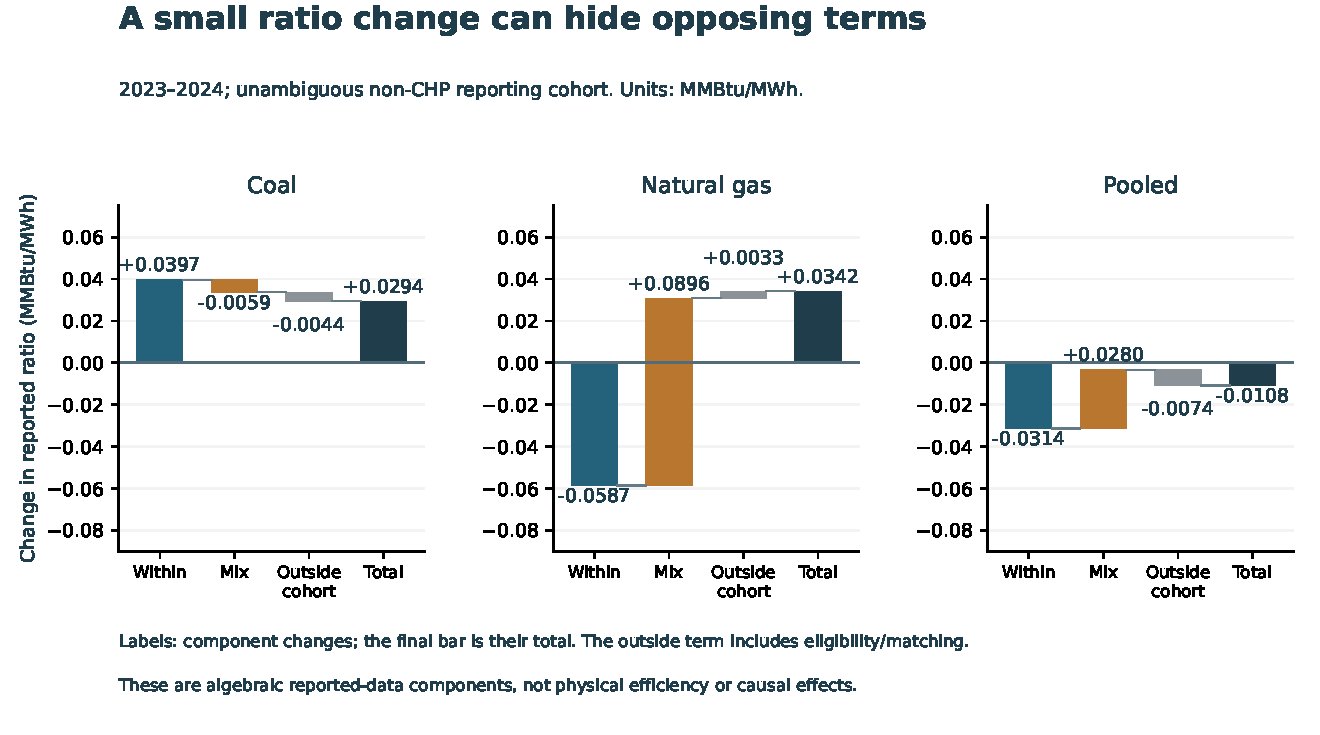
\includegraphics[width=\linewidth]{images/latest_reported_bridge.pdf}\end{center}
For the latest pooled primary case, matched generation coverage is \PooledCoverageStart{}\% and \PooledCoverageEnd{}\% of the selected eligible reporting cohort at the two endpoints. These percentages do not describe national coverage. All source decimals sum exactly; rate/share/component arithmetic uses 60 digits. Extra displayed digits describe the numerical calculation, not measurement precision. The formulas are an established algebraic identity, not a new causal attribution method.

\clearpage
\section*{3. Every grain, cohort and year-pair result}
The fixed lattice is six adjacent pairs, three fuel fleets, two grains and two matched-cohort definitions: 72 cases. Pair-common cells are eligible at both endpoints; balanced cells are eligible in all seven years. Balanced membership uses future eligibility and is a retrospective sensitivity. Development ends in 2019/2020/2021; the later summaries end in 2022/2023/2024, sharing a boundary year. There is no predictive generalization test. Thirty-seven analytical dependencies were committed at \texttt{e9acbaa8727c} before the held decomposition and influence outcomes.
\begin{center}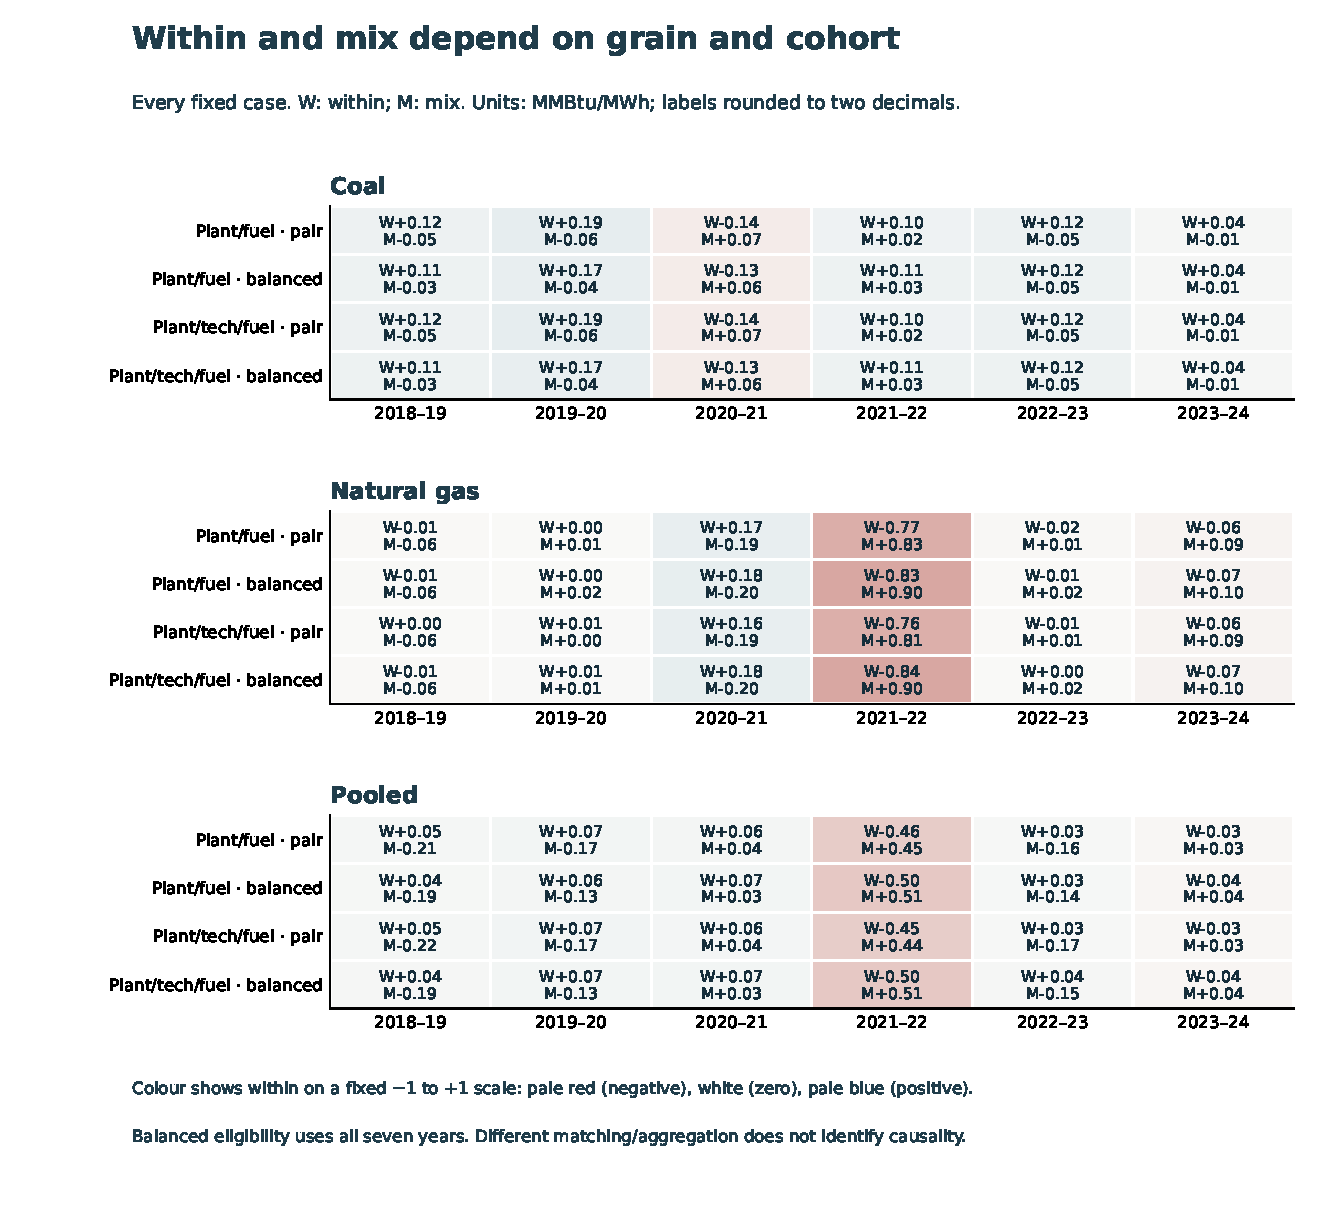
\includegraphics[width=\linewidth]{images/full_case_sensitivity.pdf}\end{center}
All \DevCases{} development and \HeldCases{} held cases are estimable. The exact source-conditional results retain both factor-order paths, endpoint totals, generation coverage and the outside-cohort remainder. No outcome, cohort, period, outlier rule or parameter changes after held inspection. No fitting, tuning, machine learning or stochastic estimation is used. The same records recur across these descriptive sensitivities.

\clearpage
\section*{4. Keep the influential-plant evidence}
Every primary case deletes each matched plant in turn, removing all its matched fuel cells. The undeleted result remains the headline result. Each line below is the finite minimum/maximum over those deletions; it is not a confidence interval or future uncertainty bound.
\begin{center}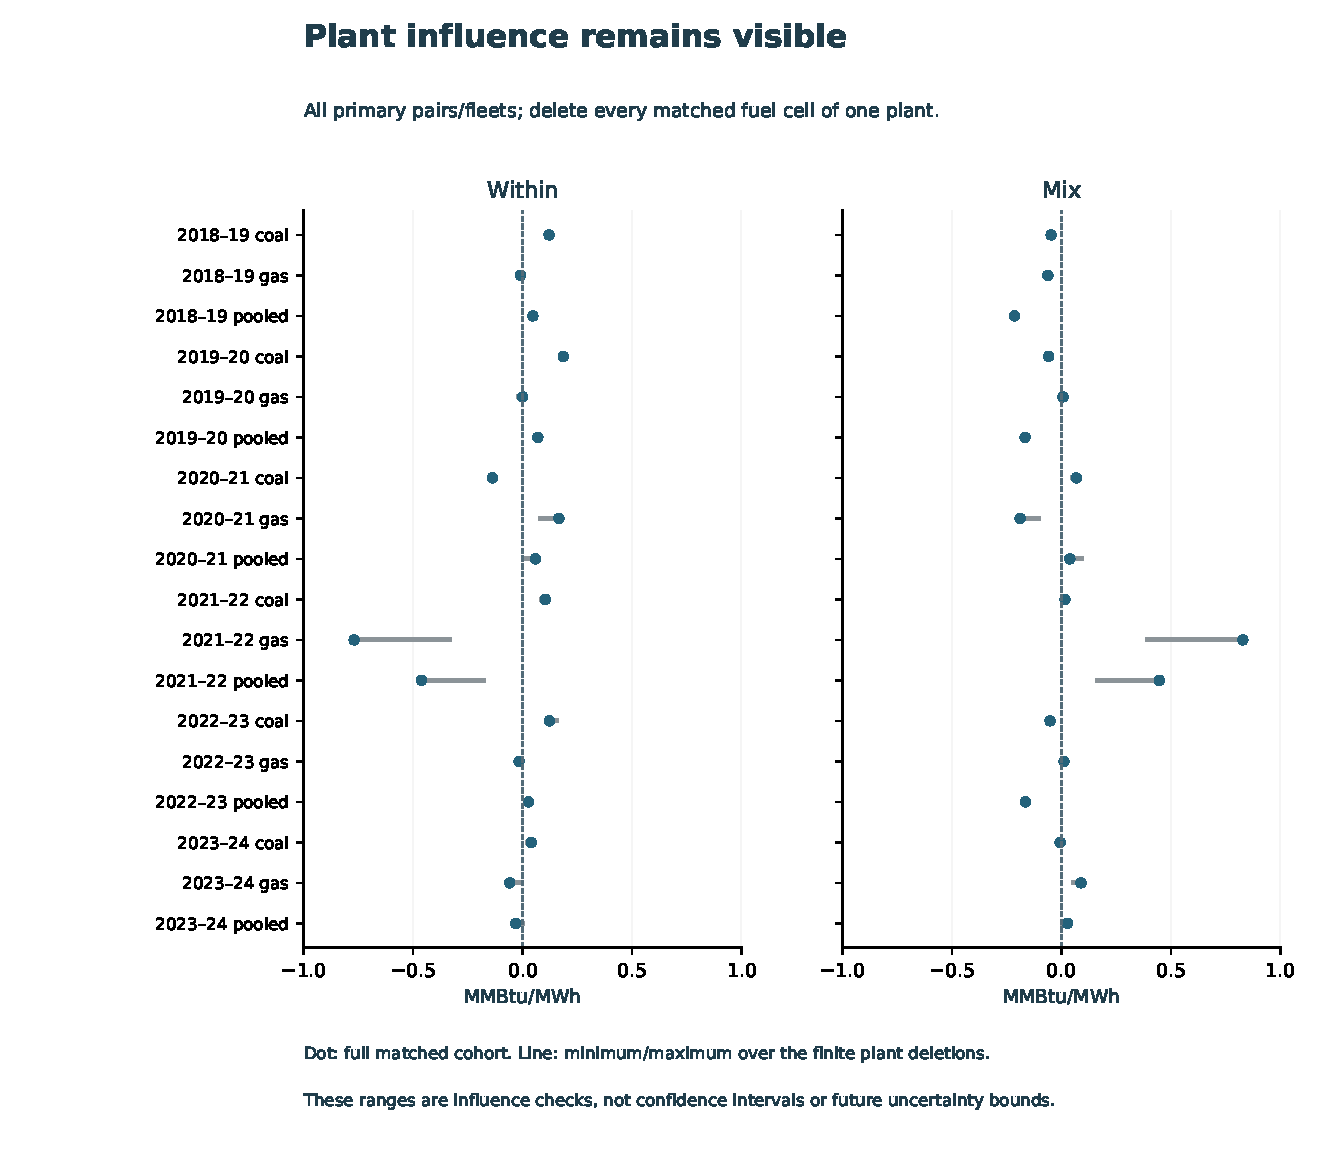
\includegraphics[width=\linewidth]{images/plant_influence_ranges.pdf}\end{center}
For 2021--2022 natural gas, within \GasOffsetWithin{} and mix \GasOffsetMix{} largely offset, while the full selected-cohort change is \GasOffsetChange{} MMBtu/MWh. The finite deletion range is material context for those large opposing terms. It does not justify an outcome-dependent plant removal. All \DevDeletions{} development and \HeldDeletions{} held deletions remain visible, with 27 direct first/middle/last recomputations in each phase supplementing the independently reconstructed subtraction sums.

The exports also retain \DevContributions{} development and \HeldContributions{} held per-case matched-cell contributions. These repeated case contributions are not additional independent source observations. Source quantities, memberships and every contribution remain traceable to the selected factual rows.

\clearpage
\section*{5. Verification, reproducibility and next evidence}
Independent openpyxl identity/classification scans and separate lxml raw-token parsing check the whole-plant quarantine and every retained source cell. There are \SourceConditions{} source/projected field conditions and \ConversionConditions{} independent numeric conversion conditions. The largest reader-conversion difference is \ConversionDifference{} against the fixed absolute $10^{-6}$ plus relative $10^{-15}$ bound. This verifies a reader conversion, not EIA measurement accuracy. Separate SQLite/80-digit Decimal grouping and membership checks pass \GroupConditions{} conditions.

The result checker imports no production aggregation or decomposition helpers. Direct 80-digit per-cell paths, path averages, matched changes and outside-cohort bridges pass \DevChecks{} development and \HeldChecks{} held conditions. It separately rebuilds all plant-subtraction quantities and recomputes the first, middle and last sorted deletion directly. The largest absolute derived-value difference is \MaxDifference{}, below the fixed $10^{-45}$ bound. Counts, memberships, keys, raw tokens and aggregated quantities are exact; derived rate/share comparisons use the declared numerical tolerance. Twenty-two authored rational/eligibility fixture methods and three authored bridge-review cases pass. These are finite numerical checks, not universal correctness or measurement validation.

Separate full-history analysis clones at \texttt{25e290a55b7e} pass on CPython 3.10.11 and 3.12.14. Each checks \ReplayExact{} exact facts and \ReplayNumeric{} derived numeric facts, with three public source files unchanged and no source request. Two as-run discrepancy diagnostics are independently bounded. Complete private workbook checks remain hash-bound; offline replay uses selected public facts and does not reacquire historical source vintages. Figures and the reviewed paper have separate source/value/geometry/artifact checks; exact final-revision Linux CI completes release validation. Variable per-case runtime records stay separate from deterministic results and are not a production-speed benchmark.

\textbf{Limits and next evidence.} The source-quality-informed quarantine excludes a fixed subset without establishing ambiguous records' overlap or a national output denominator. Annual reported cells can change with load, internal technology mix, co-fuel allocation and reporting. Aggregate ratio arithmetic cannot establish physical engineering improvement, causal effects, cost savings or retirement/entry effects. Obtain consistent unit-level allocation, technology/load histories and an appropriate measurement design before making those claims. Preserve this descriptive decomposition and all influence results as the audit layer.

\small\textbf{Sources and attribution.}\par
Source: U.S. Energy Information Administration, EIA-923 annual final historical 2018--2024 snapshots, captured 29 October 2026. Landing page: \url{https://www.eia.gov/electricity/data/eia923/}. Definitions: \url{https://www.eia.gov/survey/form/eia_923/instructions.pdf}. Reuse guidance: \url{https://www.eia.gov/about/copyrights_reuse.php}. Selection, quarantine, grouping and analysis are project transformations; no EIA endorsement is implied.\par
Exact protocol versions, full outputs, source hashes and replay: \url{https://github.com/S3R3Bii/heat-rate-composition}. Independent program manuscript, not peer reviewed; separate formal-publication projects remain private.
\end{document}
